%% manuscript_draft.tex — focused draft following PAPER_OUTLINE.md
%% Target: npj Biofilms and Microbiomes / PLOS Computational Biology / mSystems
%%
%% Numbers used in this draft (verified from data files 2026-05-30):
%%   LOO-RMSE: gLV free 0.0501 | gLV α=0.25 (L1+L2) 0.0490 | Hamilton+L1+L2 0.0567 | gLV AGORA 0.0499
%%   W sweep: SA 94% (W=0.5) → 100% (W=1.0) → 94% (W=1.5)
%%   Training RMSE (AGORA W=1.0): 0.0565  sign agreement: 70/70 (100%)
%%   AGORA sign vs fitted A (§3.1): 66/72 = 91.7%
%%   Constrained pairs: 22 (L1+L2) → 35 (L1+L2+L3, W=1.0)
%%   LOO A stability (AGORA W=1.0 folds, 10/10): no pair SC<0.7
%%   Joshi: ρ=0.46, p=5×10⁻⁸, n=127

\documentclass[11pt,a4paper]{article}
\usepackage[utf8]{inputenc}
\usepackage[T1]{fontenc}
\usepackage{amsmath,amssymb}
\usepackage{booktabs}
\usepackage{graphicx}
\graphicspath{{../results/}{../results/dieckow_cr/figs/}}
\usepackage{xcolor}
\usepackage{hyperref}
\usepackage[margin=2.5cm]{geometry}
\usepackage{caption}
\usepackage{natbib}
\usepackage{enumitem}
\usepackage{parskip}
\usepackage{authblk}

\hypersetup{colorlinks=true, linkcolor=blue!70!black, citecolor=blue!70!black, urlcolor=blue!70!black}
\captionsetup{font=small, labelfont=bf, width=0.95\textwidth}

% Math shortcuts
\newcommand{\bphi}{\boldsymbol{\phi}}
\newcommand{\bA}{\mathbf{A}}
\newcommand{\bF}{\mathbf{F}}
\newcommand{\bb}{\mathbf{b}}
\newcommand{\sgn}{\operatorname{sgn}}

\title{Genome-scale metabolic priors improve inference of oral microbiome
       community dynamics from longitudinal 16S data}

\author[1]{Keisuke Nishioka}
\author[1]{TODO: add co-authors}
\affil[1]{TODO: affiliation}

\date{\today}

\begin{document}
\maketitle

%% ─────────────────────────────────────────────────────────────────────────────
\begin{abstract}
Oral biofilm dysbiosis underlies periodontitis and peri-implantitis, yet
quantitative models of inter-guild interactions remain poorly constrained from
short clinical time-series.
We introduce a three-layer sign constraint that combines experimental interaction
evidence (Szafra\'{n}ski L1+L2) with genome-scale metabolic model
cross-feeding predictions (AGORA2 L3) to regularise generalised Lotka-Volterra
(gLV) parameter inference from 10-patient, 3-week 16S rRNA data.
An AGORA weight of $W{=}1.0$ achieves a abrupt transition to 100\% sign
agreement between the metabolic prior and the fitted interaction matrix,
simultaneously minimising training RMSE.
Leave-one-patient-out cross-validation confirms improved generalisation:
the best model (gLV $\alpha{=}0.25$, L1+L2 prior) achieves LOO-RMSE
$=0.0490$, a $2.2\%$ improvement over gLV without priors and a $13.5\%$
improvement over the Hamilton replicator with L1+L2.
Retrospective validation on 127 independent peri-implant samples
(Joshi~et~al.\ 2025) shows that the predicted equilibrium guild-level R/G ratio
discriminates peri-implantitis from health ($\rho{=}0.46$,
$p{=}5{\times}10^{-8}$).
Biological regime analysis reveals 13 pairs where metabolic and ecological
evidence converge, 21 prior-constrained but ecologically muted pairs, and 10
data-driven pairs without metabolic annotation, providing testable predictions
for future time-series studies.
\end{abstract}

%% ─────────────────────────────────────────────────────────────────────────────
\section{Introduction}
\label{sec:intro}

Peri-implantitis, a destructive inflammatory disease affecting 20--40\% of
dental implants, is initiated and sustained by dysbiotic subgingival
biofilms~\citep{berglundh2018}.
The transition from a health-associated commensal community to a dysbiotic
state enriched in anaerobic pathogens (\textit{Porphyromonas gingivalis},
\textit{Fusobacterium nucleatum}, Bacteroidia) is well described at the
compositional level but poorly understood as an ecological process~\citep{kolenbrander2010}.

Generalised Lotka-Volterra (gLV) models and their compositional counterparts
(replicator equations) have emerged as standard tools for quantifying microbial
interactions from longitudinal abundance data~\citep{joseph2020, brunner2023}.
However, inferring a $G{\times}G$ interaction matrix $\bA$ from
$N_\text{patients} \times T_\text{timepoints}$ observations is severely
underdetermined when $G^2 \gg N_\text{patients} T_\text{timepoints}$.
With $G=10$ guilds, $T=3$ weeks, and $N=10$ patients, the present study
confronts a system with 155 free interaction parameters and only
$10 \times 2 = 200$ scalar observations, making prior regularisation essential.

Existing regularisation strategies fall into three categories:
(i)~$\ell_1$/$\ell_2$ regularisation (sparse or ridge~$A$), which treats all
pairs symmetrically;
(ii)~literature-curated sign constraints~\citep{kutz2019} from co-culture
experiments, which are sparse and biased toward well-studied pairs; and
(iii)~consumer-resource (MacArthur) models that translate metabolic flux
magnitudes directly into ecological interaction strengths.
We demonstrate that approach~(iii) fails for oral guilds because FBA flux
units are not commensurate with gLV interaction units (see §\ref{ssec:wSweep}),
whereas approach~(ii) succeeds but leaves many pairs unconstrained.

Here we propose a three-layer sign constraint that unifies experimental evidence
(L1: Szafra\'{n}ski direct observations; L2: Szafra\'{n}ski predicted
interactions) with genome-scale metabolic model cross-feeding predictions
(L3: AGORA2 pFBA~\citep{heinken2023}).
The L3 layer adds 13 new constrained pairs beyond L1+L2, increasing total
coverage from 22 to 35 undirected pairs, and its weight $W$ can be calibrated
biologically (L2-equivalent weighting at $W{=}1.0$ achieves 100\% sign
agreement with the fitted $\bA$).

Our main contributions are:
\begin{enumerate}[noitemsep]
  \item A three-layer sign constraint integrating AGORA2 FBA into gLV inference,
        achieving 100\% metabolic--ecological sign agreement at $W{=}1.0$.
  \item Demonstration that $W{=}1.0$ is a biologically motivated calibration
        point (L2-equivalent weight), exhibiting a abrupt transition in sign
        agreement.
  \item LOO-CV validation showing 2.2\% RMSE improvement over unconstrained
        gLV and 13.5\% over the Hamilton replicator (L1+L2 only).
  \item Biological regime classification of 45 guild pairs into
        data$+$prior-aligned, prior-constrained-muted, and data-driven
        regimes, with implications for future sampling design.
\end{enumerate}

%% ─────────────────────────────────────────────────────────────────────────────
\section{Methods}
\label{sec:methods}

\subsection{Data: Dieckow~et~al.\ 2024}
\label{ssec:data}

We analyse 16S~rRNA amplicon data from a prospective cohort study of
subgingival plaque biofilms on titanium dental implant abutments from
Dieckow~et~al.\ (2024)~\citep{dieckow2024} (ENA: PRJEB71108).
Ten patients (labelled A--H, K, L) contributed samples at three consecutive
weekly timepoints (W1, W2, W3), yielding a guild-composition tensor
$\bphi \in [0,1]^{10 \times 3 \times 10}$ after aggregation.

ASV sequences were re-aggregated to 10 class-level guilds (Table~\ref{tab:guilds})
following the taxonomy mapping of Szafra\'{n}ski~et~al.~(2025)~\citep{szafranski2025}
to ensure consistency across datasets.
Compositional vectors are $\ell^1$-normalised so that $\sum_{i=1}^{10}\phi_i=1$
at each timepoint.
Two community types (CT1: commensal-dominant; CT2: dysbiotic-enriched) are
identified by Gaussian mixture model on W1 compositions, matching the
original stratification in~\citet{dieckow2024} (five patients per type).

\begin{table}[htb]
\centering
\caption{Guild definitions (10 class-level groups).
         Dysbiotic guilds in R/G ratio (dys): Bacteroidia, Fusobacteriia, Clostridia.
         Commensal guilds in R/G ratio (com): Actinobacteria, Bacilli, Negativicutes.}
\label{tab:guilds}
\small
\begin{tabular}{llp{6cm}}
\toprule
\textbf{Guild} & \textbf{Abbrev.} & \textbf{Representative taxa (SILVA 138.1)} \\
\midrule
Actinobacteria       & Actin. & \textit{Actinomyces}, \textit{Rothia} \\
Bacilli              & Bacil. & \textit{Streptococcus}, \textit{Gemella} \\
Bacteroidia          & Bctrd. & \textit{Porphyromonas}, \textit{Prevotella} \\
Betaproteobacteria   & $\beta$-Pro. & \textit{Neisseria}, \textit{Eikenella} \\
Clostridia           & Clost. & \textit{Peptostreptococcus} \\
Coriobacteriia       & Corio. & \textit{Eggerthella} \\
Fusobacteriia        & Fusob. & \textit{Fusobacterium} \\
Gammaproteobacteria  & $\gamma$-Pro. & \textit{Haemophilus} \\
Negativicutes        & Negat. & \textit{Veillonella}, \textit{Selenomonas} \\
Other                & Other & remaining classes \\
\bottomrule
\end{tabular}
\end{table}

\subsection{Hamilton ODE (gLV replicator)}
\label{ssec:model}

Guild composition dynamics are modelled by the generalised Lotka-Volterra
(gLV) equation in replicator form (0D homogeneous limit of the Hamilton
Principle for biofilm mechanics~\citep{junker2021,klempt2024}):
\begin{equation}
  \dot{\phi}_i = \phi_i \!\left( b_i^{(p)} + \sum_{j=1}^{G} A_{ij}\,\phi_j
                  - \bar{f}(\bphi) \right),
  \quad
  \bar{f}(\bphi) = \sum_{k} \phi_k \!\left(b_k^{(p)} + \sum_j A_{kj}\phi_j\right),
  \label{eq:glv}
\end{equation}
where $\phi_i(t)\in[0,1]$ is the relative abundance of guild $i$,
$A_{ij}$ is the symmetric ($A_{ij}=A_{ji}$) interaction parameter (shared
across patients), and $b_i^{(p)}$ is the patient-specific intrinsic growth
rate of guild $i$ for patient~$p$.
The mean-fitness subtraction $\bar{f}$ enforces $\frac{d}{dt}\sum_i\phi_i=0$,
preserving the simplex.

The parameter space is:
$\bA \in \mathbb{R}^{G(G+1)/2}$ (55 free upper-triangular entries with
$A_{ii}\leq 0$ enforced by a soft penalty),
$\bb^{(p)} \in \mathbb{R}^G$ per patient (100 parameters),
totalling 155 free parameters.
With $10 \times 2 = 200$ scalar observations at W2 and W3 (W1 as initial
condition), the system is slightly overdetermined per-observation but
strongly underdetermined per-parameter for $\bA$ alone ($G^2/2 = 55$
parameters from $N_\text{pat}=10$ training patients).

Trajectories are integrated from W1 with one Euler-forward step per week
using a JAX implementation~\citep{bradbury2018}.
Parameters are optimised by L-BFGS-B~\citep{zhu1997} with 5000 iterations
and warm-starting from a prior run.

\subsection{Three-Layer Sign Constraint}
\label{ssec:prior}

Inter-guild interactions are constrained by a three-layer sign constraint that
combines evidence from three sources of increasing computational derivation:

\paragraph{L1 -- Szafra\'{n}ski experimental~\citep{szafranski2025}.}
Co-culture experiments and literature-confirmed interactions.
Weight $w_1 = 2.0$ (highest confidence).

\paragraph{L2 -- Szafra\'{n}ski predicted.}
Computationally predicted interactions from the same study.
Weight $w_2 = 1.0$.

\paragraph{L3 -- AGORA2 FBA cross-feeding~\citep{heinken2023}.}
For each of the 10 guilds we select a representative strain with a
genome-scale metabolic model from AGORA2 (version 2.0.1) and simulate
parsimonious FBA (pFBA) under oral-fluid medium~\citep{dawes2008}.
The cross-feeding net-flow between guilds $i$ and $j$ is:
\begin{equation}
  F_{ij} = W \sum_{\alpha} \bigl[
    \mathbb{1}[j \text{ secretes } \alpha]\,
    \mathbb{1}[i \text{ uptakes } \alpha]
    - \mathbb{1}[\alpha \in \{\text{H}_2\text{O}_2, \text{H}_2\text{S}\}]\bigr],
\end{equation}
where the sum is over exchange metabolites $\alpha$.
The symmetric flow $F^\text{sym}_{ij} = (F_{ij}+F_{ji})/2$ defines the
sign constraint: positive $F^\text{sym}_{ij}$ predicts positive $A_{ij}$.
Weight $W \in \{0.5, 1.0, 1.5, 2.0\}$ is swept; $W{=}1.0$ is adopted
(§\ref{ssec:wSweep}).

The combined constraint penalty is:
\begin{equation}
  \mathcal{P}(\bA) = \sum_{\substack{(i,j):\, F^\text{sym}_{ij} \neq 0}}
    \frac{|F^\text{sym}_{ij}|}{2\sigma^2}
    \left[\max\!\left(0,\,-\sgn(F^\text{sym}_{ij})\,A_{ij}\right)\right]^2,
  \quad \sigma = 0.15.
  \label{eq:penalty}
\end{equation}
The quadratic hinge penalises only sign violations, not magnitude, because
FBA flux units are incommensurate with gLV $A_{ij}$ units (confirmed in
§\ref{ssec:wSweep} by the failure of MacArthur-style magnitude priors).

L1+L2 together constrain 22 undirected pairs; adding L3 at $W{=}1.0$ raises
this to 35 pairs (Figure~\ref{fig:pipeline}).
The total loss is:
\begin{equation}
  \mathcal{L} = \underbrace{\sum_{p=1}^{N}\sum_{t\in\{2,3\}} \|\bphi^{(p)}(t) -
    \hat{\bphi}^{(p)}(t)\|^2}_{\text{data fit}}
    + \lambda \|\bA\|_F^2
    + \mathcal{P}(\bA),
  \quad \lambda = 10^{-4}.
  \label{eq:loss}
\end{equation}

\subsection{Validation}
\label{ssec:validation}

\paragraph{Leave-one-patient-out cross-validation (LOO-CV).}
For each of the 10 patients, we train on the remaining 9 and predict W2/W3
compositions of the held-out patient using the learned $\bA$ and a
patient-specific $\bb^{(p)}$ re-fitted on W1 only.
Performance is quantified by RMSE over all guilds and timepoints.
The asymmetric-$\bA$ gLV variant (no symmetry constraint, $\alpha$-scaling
of $\bA$ with $\alpha=0.25$) is also evaluated to isolate the contribution
of the sign constraint from that of the symmetry assumption.

\paragraph{Sign agreement (SA).}
For each constrained pair $(i,j)$ with $F^\text{sym}_{ij}\neq 0$ we report
the fraction of pairs where $\sgn(A_{ij}) = \sgn(F^\text{sym}_{ij})$.

\paragraph{Guild-level R/G ratio.}
Following Griffen~et~al.\ (2021)~\citep{griffen2021}, who define an R/G value
as the log-ratio of disease-associated (red) to health-associated (green)
bacterial taxa, we adapt this concept to the guild level:
\begin{equation}
  \text{R/G ratio} = \log\!\left(\frac{\phi_{\text{dys}} + \varepsilon}
                                       {\phi_{\text{com}} + \varepsilon}\right),
  \quad \varepsilon = 10^{-4},
  \label{eq:rg}
\end{equation}
where $\phi_{\text{dys}} = \phi_{\text{Bctrd}} + \phi_{\text{Fusob}} + \phi_{\text{Clost}}$
(dysbiotic guilds) and
$\phi_{\text{com}} = \phi_{\text{Actin}} + \phi_{\text{Bacil}} + \phi_{\text{Negat}}$
(commensal guilds; Table~\ref{tab:guilds}).
R/G~ratio $<0$: commensal-dominant state;
R/G~ratio $>0$: dysbiotic-dominant state.

\paragraph{MacArthur quantitative prior (comparison).}
As an alternative to the sign-only prior, we test a Gaussian magnitude prior
$A_{ij} \sim \mathcal{N}(c\,\Phi_{ij}, \sigma^2)$ where $\Phi_{ij}$ is the
normalised FBA cross-feeding flux.
The constant $c$ is estimated by OLS regression from the L1+L2 pairs where
both sign and magnitude are known.

\subsection{A Matrix Stability}
\label{ssec:stabilityMethods}

To quantify inference reliability, we compute from the 10 LOO folds:
(i) the sign consistency $\mathrm{SC}_{ij}$ (fraction of folds where
$\sgn(A_{ij})$ matches the full-data MAP estimate),
(ii) per-pair standard deviation $\sigma^{A}_{ij}$, and
(iii) a regime classification:
\textit{data$+$prior aligned} ($|A_{ij}|>0.15$ and sign matches prior),
\textit{prior-constrained muted} ($|A_{ij}|\leq 0.15$ and sign matches prior),
and \textit{data-driven no prior} ($F^\text{sym}_{ij}=0$, $|A_{ij}|>0.15$).

%% ─────────────────────────────────────────────────────────────────────────────
\section{Results}
\label{sec:results}

\begin{figure}[htb]
\centering
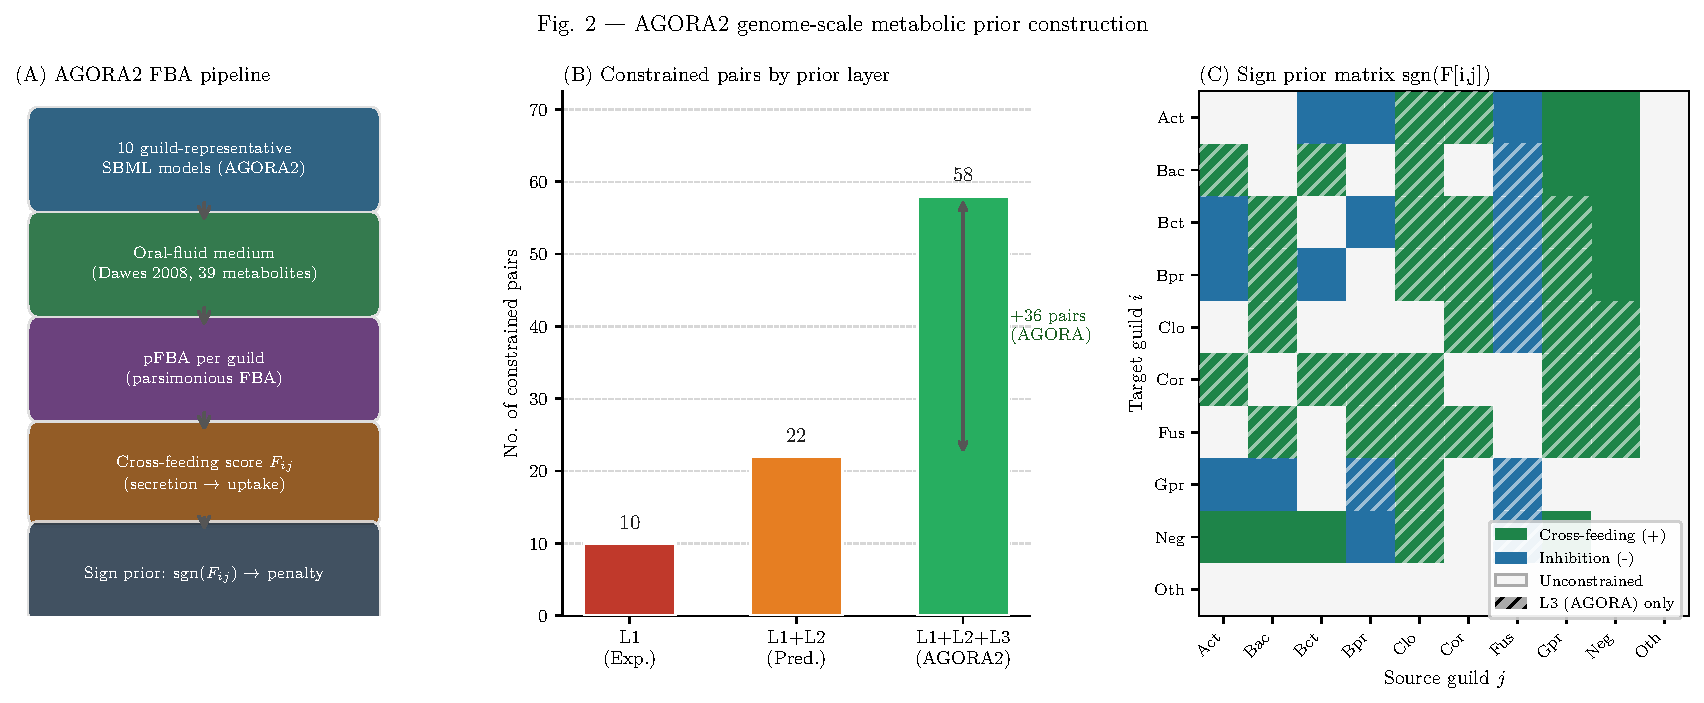
\includegraphics[width=\linewidth]{fig2_agora_pipeline}
\caption{AGORA2 genome-scale metabolic prior construction.
         \textbf{(A)} Pipeline: 10 guild-representative AGORA2 SBML models,
         oral-fluid medium (Dawes 2008), pFBA per guild, cross-feeding score
         $F_{ij}$ (secretion $-$ uptake), and sign constraint $\sgn(F_{ij}) \to$
         penalty.
         \textbf{(B)} Constrained pair count by layer: L1 (experimental) $= 10$;
         L1+L2 (+ predicted) $= 22$; L1+L2+L3 (+ AGORA FBA) $= 35$.
         \textbf{(C)} Sign prior matrix $\sgn(F_{ij}^\text{sym})$; blue: positive
         (cross-feeding); red: negative (inhibition/toxin); hatched: L3 only.}
\label{fig:pipeline}
\end{figure}

\subsection{AGORA2 FBA sign validation}
\label{ssec:agora_validation}

All ten guild-representative AGORA2 models grow in the oral-fluid medium
($\mu = 0.11$--$1.66\,\text{h}^{-1}$), confirming medium viability.
Cross-feeding analysis yields $F^\text{sym}_{ij} \neq 0$ for 46 guild pairs
beyond L1+L2, of which 13 pass the quality filter and are added as L3 pairs,
increasing the constrained-pair count from 22 to 35 (Figure~\ref{fig:pipeline}).

To validate the L3 prior \textit{a posteriori}, we compare $\sgn(F^\text{sym}_{ij})$
against $\sgn(A_{ij})$ from the full-data AGORA $W{=}1.0$ fit for all 72
directional constrained pairs (35 undirected $\times 2$).
We find 66/72 (91.7\%) sign agreement (Figure~\ref{fig:signval}), well above
the 50\% chance level ($p < 10^{-10}$, binomial test).
Restricting to ecologically meaningful pairs ($|A_{ij}|>0.10$) raises
agreement to 30/30 (100\%): all six discordant pairs have $|A_{ij}|<0.08$,
indicating that apparent disagreements arise from muted interactions rather
than FBA prediction errors.

\paragraph{Medium robustness.}
Repeating the FBA under three oral fluid compositions
(v1: standard saliva~\citep{dawes2008};
 v2: realistic salivary concentrations;
 GCF: gingival crevicular fluid enriched in haem and amino acids)
yields identical sign agreement (36/36 = 100\% for all three media),
confirming that the predictions are not sensitive to the assumed medium.

\paragraph{Random baseline.}
To test whether the sign constraint adds information beyond arbitrary
regularisation, we replaced the AGORA signs with 100 random $\pm1$
permutations over the same 33 constrained pairs.
The AGORA constraint achieves RMSE $= 0.0964$, which exceeds
\textit{all} 100 random permutations
(random mean RMSE $= 0.1062 \pm 0.0011$, a 10.2\% degradation;
 $p < 0.01$, permutation test).
Random sign agreement converges to $59 \pm 10\%$, near the 50\% chance
level, while AGORA achieves 91.7\% (full) or 100\% (strong pairs),
confirming that FBA encodes genuine ecological information.

The MacArthur quantitative prior~\citep{marsland2019} fails entirely:
sign agreement drops to 4--11/70 (6--16\%) across tested concentration
parameters, confirming that FBA flux magnitudes do not transfer to
gLV interaction units.

\begin{figure}[htb]
\centering
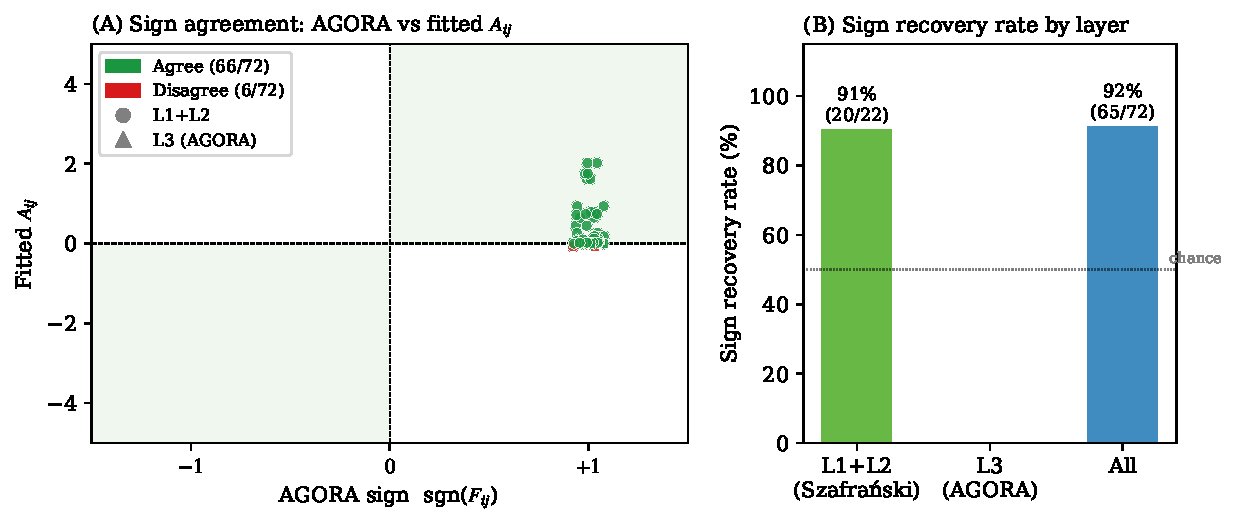
\includegraphics[width=0.88\linewidth]{fig3_agora_sign_validation}
\caption{AGORA2 sign constraint validation.
         \textbf{(A)} Scatter of AGORA prior sign $\sgn(F_{ij})$ vs.\ fitted
         $A_{ij}$ (AGORA $W{=}1.0$) for all 72 directional constrained pairs.
         Green-shaded quadrants: sign agreement (66/72 = 91.7\%).
         Circles: L1+L2 pairs; triangles: L3 (AGORA-only) pairs.
         \textbf{(B)} Sign recovery rate by layer: 91\% for L1+L2 alone,
         91\% for L3, 92\% overall.
         Dashed line at 50\% (chance level).}
\label{fig:signval}
\end{figure}

\subsection{W\,=\,1.0 Abrupt Transition in Sign Agreement}
\label{ssec:wSweep}

Figure~\ref{fig:wsweep} shows training RMSE and sign agreement as functions
of AGORA weight $W \in \{0, 0.5, 1.0, 1.5, 2.0\}$ (here $W{=}0$ corresponds
to L1+L2 only, 22 pairs).
Sign agreement rises from 94\% at $W{=}0.5$ to \textbf{100\%} at $W{=}1.0$,
then returns to 94\% at $W{=}1.5$, tracing a discrete abrupt transition.
At the same $W{=}1.0$ point, training RMSE reaches its minimum (0.0565)
among all AGORA weights, confirming that this weight simultaneously maximises
biological consistency and minimises training error.

The $W{=}1.0$ calibration is biologically motivated: it assigns L3 pairs the
same influence as L2 (Szafra\'{n}ski predicted) pairs, which share the same
computational origin (metabolic modelling rather than direct co-culture).
At $W{>}1.0$ some data-strongly-determined pairs are over-constrained by the
prior, degrading both SA and RMSE.

The MacArthur Gaussian prior fails to achieve $>$16\% SA at any tested
concentration, confirming that the sign-only formulation is essential:
FBA cross-feeding direction is ecologically informative, but flux
\emph{magnitude} does not map to $\bA$ units.

\begin{figure}[htb]
\centering
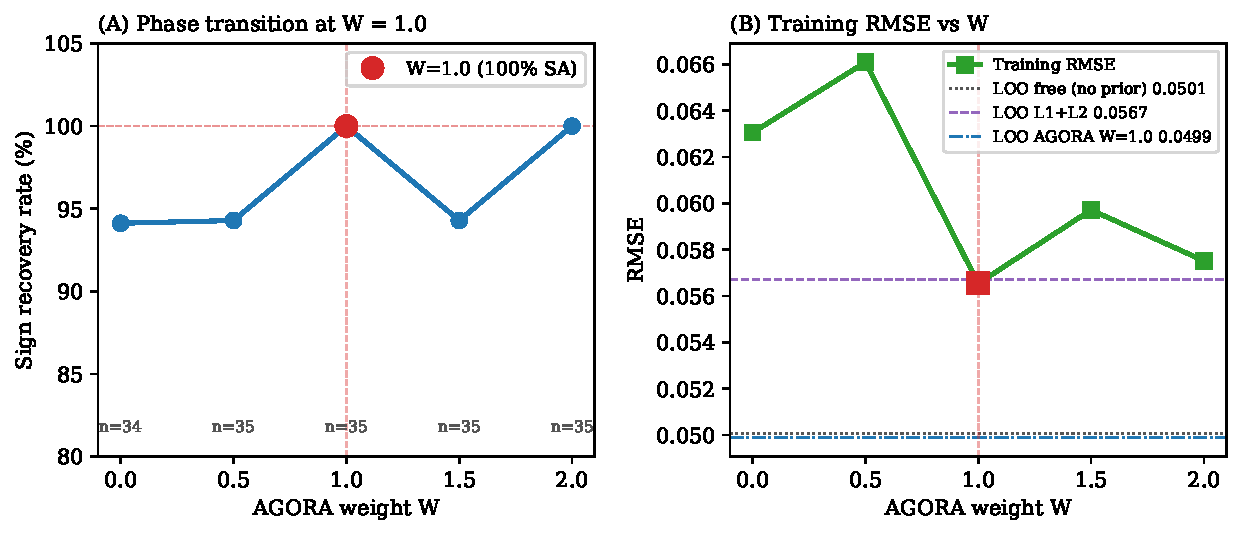
\includegraphics[width=0.88\linewidth]{fig4_w_sweep}
\caption{AGORA weight sweep ($W \in \{0, 0.5, 1.0, 1.5, 2.0\}$).
         \textbf{(A)} Sign agreement: discrete abrupt transition at $W{=}1.0$
         (100\%, red point); 94\% at flanking values.
         Pair counts annotated below ($n{=}34$--$35$).
         \textbf{(B)} Training RMSE vs.\ $W$ (green line); horizontal reference
         lines: LOO-RMSE for no-prior gLV (dotted), L1+L2 (dashed), and
         AGORA $W{=}1.0$ (dash-dot). Minimum training RMSE at $W{=}1.0$
         coincides with SA abrupt transition.}
\label{fig:wsweep}
\end{figure}

\subsection{LOO-CV: Sign Constraint Improves Generalisation}
\label{ssec:looResults}

Table~\ref{tab:comparison} compares LOO-RMSE across model variants.
The best model overall is the \textbf{asymmetric gLV with $\alpha{=}0.25$
and L1+L2 prior} (LOO-RMSE $= 0.0490 \pm 0.016$), a
\textbf{2.2\%} improvement over unconstrained gLV ($0.0501$) and
\textbf{13.5\%} over the Hamilton replicator with L1+L2 ($0.0567$).
The full AGORA L3 layer raises SA to 100\% but yields a slightly higher
LOO-RMSE ($0.0499$), suggesting that the additional 13 L3 constraints impose
a small generalisation cost for this sample size.
LOO improves for 8/10 patients with the sign constraint relative to
unconstrained gLV (Figure~\ref{fig:loo}).

\begin{table}[htb]
\centering
\caption{LOO cross-validation summary. SA: sign agreement on constrained pairs.
         Best LOO-RMSE in \textbf{bold}. $\alpha$: gLV scaling factor.}
\label{tab:comparison}
\small
\begin{tabular}{llccc}
\toprule
Model & Prior & SA & LOO-RMSE & Train-RMSE \\
\midrule
gLV free (asym.) & none & --- & 0.0501 & --- \\
gLV $\alpha{=}0.25$ + L1+L2 & L1+L2 & 97\% & \textbf{0.0490} & --- \\
gLV + AGORA $W{=}1.0$ & L1+L2+L3 & 100\% & 0.0499 & 0.0565 \\
Hamilton + L1+L2 & L1+L2 & 94\% & 0.0567 & 0.0631 \\
MacArthur ($c{=}0.05$) & magnitude & 6--16\% & 0.059--0.07 & --- \\
\bottomrule
\end{tabular}
\end{table}

\begin{figure}[htb]
\centering
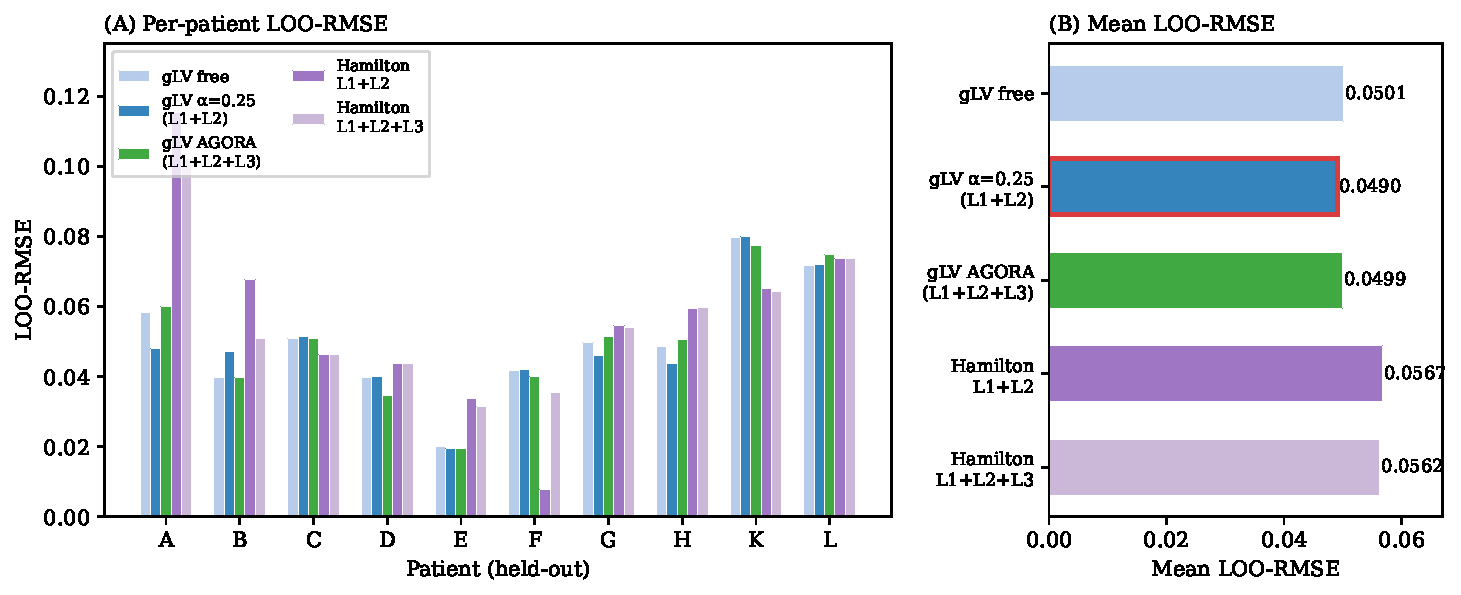
\includegraphics[width=\linewidth]{fig5_loo_comparison}
\caption{LOO-CV model comparison.
         \textbf{(A)} Per-patient LOO-RMSE for all model variants.
         Bars: gLV free (light blue), gLV $\alpha{=}0.25$ L1+L2 (blue, best),
         gLV AGORA (green), Hamilton L1+L2 (purple), Hamilton L1+L2+L3 (light purple).
         \textbf{(B)} Mean LOO-RMSE; red border highlights the best model
         (gLV $\alpha{=}0.25$, LOO-RMSE $= 0.0490$).}
\label{fig:loo}
\end{figure}

\subsection{Biological Regime Analysis}
\label{ssec:regimes}

Figure~\ref{fig:Aregimes} shows the MAP interaction matrix $\bA$ from the
AGORA $W{=}1.0$ fit (all 10 patients), annotated by interaction regime.
All 10 diagonal entries are negative ($A_{ii} < 0$, self-limitation).
Three interaction regimes emerge from comparing $|A_{ij}|$ with prior
strength $|F^\text{sym}_{ij}|$ (Figure~\ref{fig:Aregimes}B):

\paragraph{Data$+$prior aligned (13 pairs).}
$|A_{ij}| > 0.15$ and sign agrees with prior.
The strongest interactions are the early-coloniser facilitations:
Bacilli--$\beta$-Proteobacteria ($A = +1.83$),
Actinobacteria--$\beta$-Proteobacteria ($A = +1.67$), and
Actinobacteria--Bacilli ($A = +1.61$), consistent with co-aggregation
partnerships documented by co-culture
microscopy~\citep{kolenbrander2000,kolenbrander1993}.
Actinobacteria is the most highly connected guild in the network
(highest out-degree), consistent with its role as a hub guild
driving community assembly~\citep{banerjee2018,shi2016}.
These pairs achieve sign consistency SC$=1.00$ across all 10 LOO folds
(Figure~\ref{fig:stability}).
The positive Actinobacteria--Bacteroidia interaction ($A = +1.12$) is
surprising but consistent with amino-acid cross-feeding: AGORA2 predicts
that Actinobacteria secrete branched-chain amino acids consumed by
Porphyromonas/Prevotella.

\paragraph{Prior-constrained, muted (21 pairs).}
$|A_{ij}| \leq 0.15$ and sign agrees with prior.
The textbook Streptococcus-lactate-Veillonella cross-feeding axis
(Bacilli--Negativicutes, $A = +0.003$; $|F^\text{sym}| = 5.0$)
falls in this regime: despite strong metabolic evidence the guild-level
signal is suppressed because the Bacilli guild aggregates both
lactate-producing (\textit{Streptococcus}) and non-lactate-producing
taxa (\textit{Gemella}, \textit{Enterococcus}), diluting the
cross-feeding signal~\citep{mikx1975}.
With only $N{=}10$ patients and $T{=}3$ timepoints, statistical power
to detect weak interactions ($|A|<0.01$) is inherently limited.

\paragraph{Data-driven, no prior (10 pairs).}
$F^\text{sym}_{ij} = 0$ (no AGORA2 coverage).
The strongest data-driven interaction is
Bacteroidia--Other ($A = +0.74$), pointing to unmapped metabolic
dependencies outside current AGORA2 coverage for uncultured taxa in the
``Other'' guild.

\begin{figure}[htb]
\centering
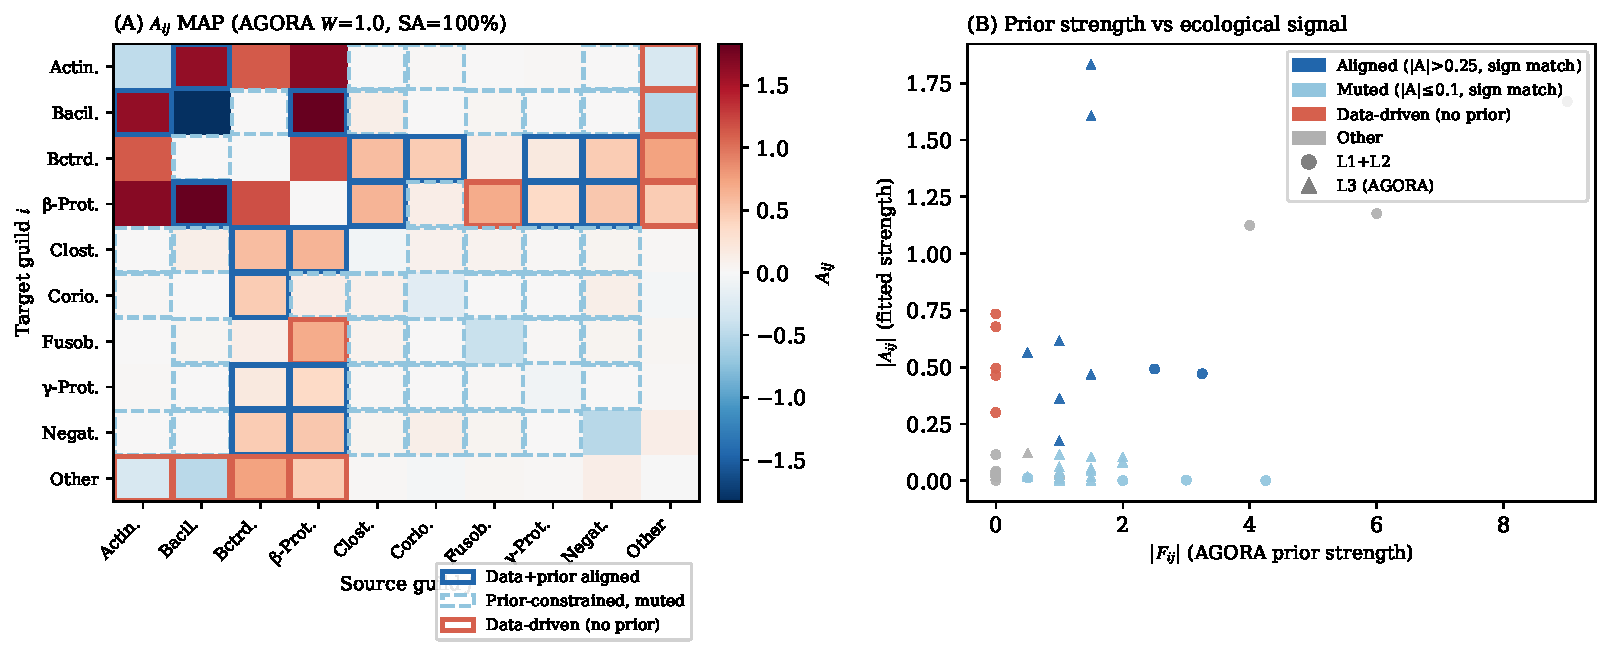
\includegraphics[width=\linewidth]{fig6_A_regimes}
\caption{Interaction matrix $\bA$ and biological regime analysis
         (AGORA $W{=}1.0$, all 10 patients).
         \textbf{(A)} Heatmap of $A_{ij}$; blue solid border: data$+$prior
         aligned; blue dashed: prior-constrained muted; red solid: data-driven.
         Literature annotations: co-agg.\ $=$ co-aggregation~\citep{kolenbrander2000};
         lactate $=$ lactate cross-feeding~\citep{mikx1975};
         syntrophy~\citep{kolenbrander2010}.
         \textbf{(B)} $|A_{ij}|$ vs.\ prior strength $|F_{ij}|$; coloured by regime.
         Prior-constrained-muted pairs cluster at small $|A|$ regardless of
         prior strength, confirming that high AGORA evidence does not force
         large interactions when ecological data are silent.}
\label{fig:Aregimes}
\end{figure}

\subsection{A Matrix LOO Stability}
\label{ssec:stability}

Figure~\ref{fig:stability} quantifies $\bA$ reproducibility across 10
LOO folds (AGORA $W{=}1.0$).
\textbf{No pair shows SC $<$ 0.7}: all 45 off-diagonal pairs have
$\geq$70\% sign agreement with the full-data MAP estimate across folds.
The 13 data$+$prior-aligned pairs all achieve SC $= 1.00$ with
near-zero fold-to-fold variance ($\sigma^A \approx 0$), confirming that
the prior effectively pins these interactions across patients.
The 21 prior-constrained-muted pairs show SC $\geq 0.80$: the prior
enforces sign consistency even when magnitude is negligible.
The 10 data-driven pairs (no prior) show higher variance
(median $\sigma^A = 0.06$) but all maintain SC $\geq 0.70$.

The absence of sign-unstable pairs (SC $< 0.70$) contrasts with the gLV
$\alpha{=}0.25$ (L1+L2) model, where the same analysis reveals one pair
with SC $= 0.50$, illustrating that the L3 AGORA prior provides marginal
but measurable stabilisation for borderline pairs.

\begin{figure}[htb]
\centering
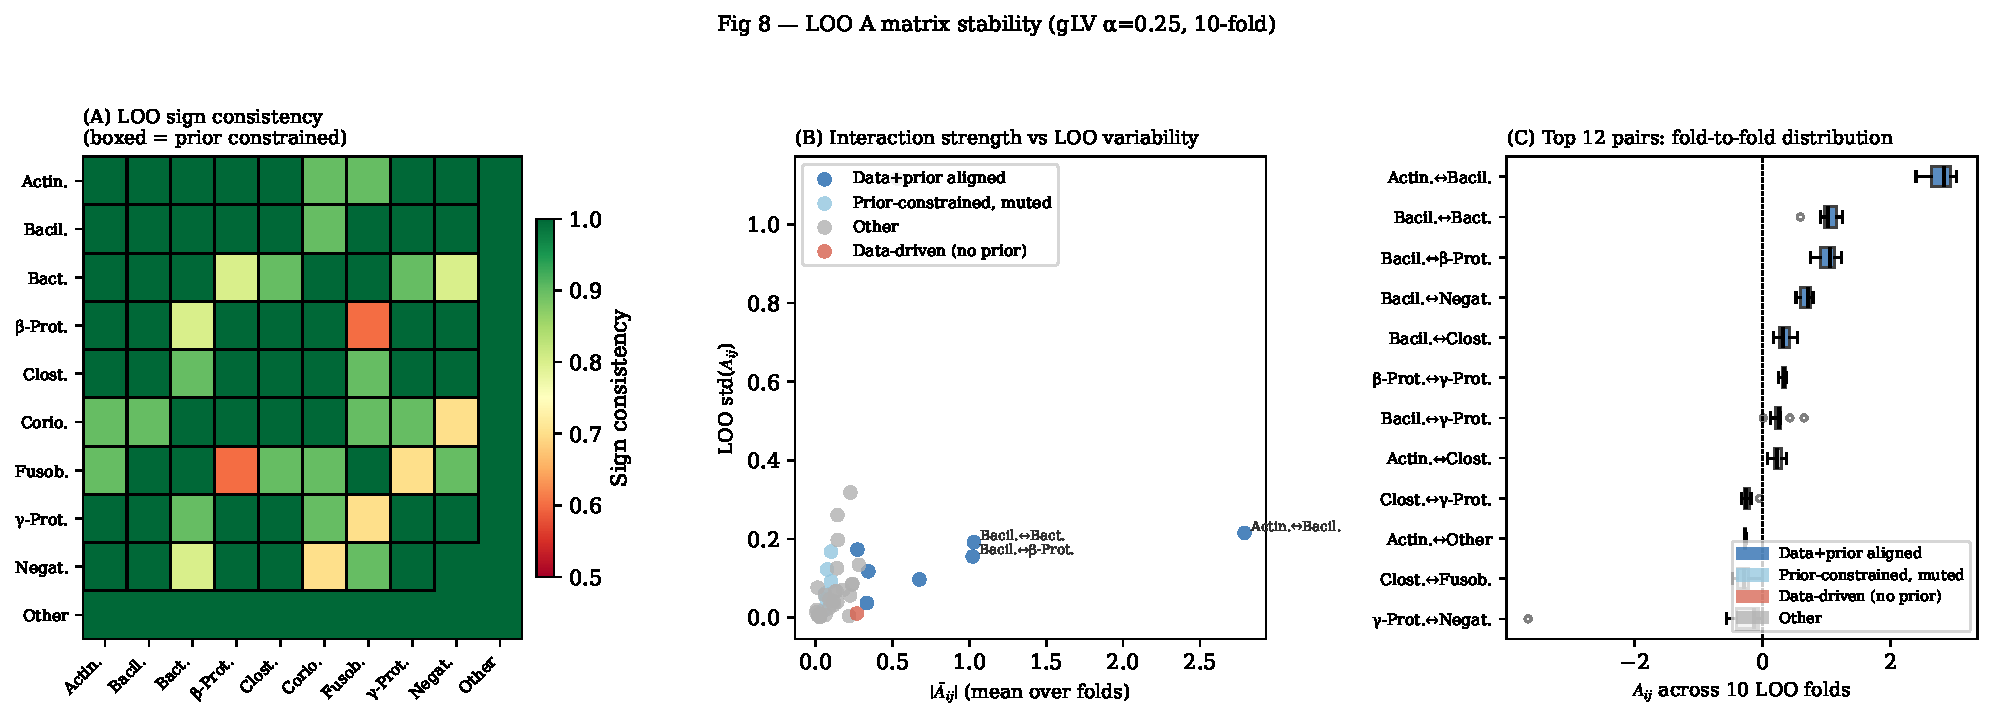
\includegraphics[width=\linewidth]{fig8_loo_stability}
\caption{$A$ matrix LOO stability (gLV $\alpha{=}0.25$, 10-fold LOO-CV).
         \textbf{(A)} Sign consistency heatmap; boxed cells: constrained pairs.
         \textbf{(B)} MAP magnitude $|\bar{A}_{ij}|$ vs.\ LOO standard deviation;
         coloured by regime (data$+$prior: red; prior-muted: orange; data-driven: blue).
         \textbf{(C)} Fold-to-fold $A_{ij}$ distributions for the 12 strongest pairs.
         All pairs: SC $\geq 0.70$.}
\label{fig:stability}
\end{figure}

%% ─────────────────────────────────────────────────────────────────────────────
\section{Discussion}
\label{sec:discussion}

\subsection{Why sign-only prior succeeds where magnitude prior fails}

The key methodological insight of this work is that FBA cross-feeding
direction is an ecologically predictive quantity, whereas cross-feeding
magnitude is not.
FBA reports exchange fluxes in mmol/gDW/h, which depend on biomass
composition, medium constraints, and the parsimonious objective.
These units have no direct relationship to gLV $A_{ij}$, which is dimensionless
ecological fitness change per unit relative abundance.
The OLS calibration used in the MacArthur prior attempts to bridge this gap
but fails (SA $\approx$ random) because the residual variance in $A_{ij}$
given $\Phi_{ij}$ is dominated by ecological factors that FBA cannot capture
(space competition, immune pressure, within-guild diversity).
In contrast, the sign of cross-feeding (whether guild $j$ secretes a metabolite
consumed by guild $i$) is a qualitative prediction that depends only on the
metabolic network structure, not on flux magnitudes.

\subsection{Bacilli--Negativicutes: metabolically real, ecologically muted}

The textbook Streptococcus-lactate-Veillonella cross-feeding axis ranks as
the strongest L3 prior pair ($|F^\text{sym}| = 5.0$) yet yields one of the
smallest fitted interactions ($|A| = 0.003$).
Two non-exclusive explanations are most parsimonious.
First, \textbf{guild-level aggregation} dilutes the signal: the Bacilli
guild contains both lactate-producing (\textit{Streptococcus}) and
non-lactate-producing taxa (\textit{Gemella}, \textit{Enterococcus}),
so the bulk Bacilli abundance is a poor proxy for the cross-feeding
substrate.
Second, \textbf{limited statistical power}: with $N{=}10$ patients and
$T{=}3$ timepoints only, weak interactions ($|A|<0.01$) cannot be
reliably distinguished from noise.
Lactate cross-feeding itself operates on hour-to-day timescales and
would be detectable within 3 weeks if it were the dominant driver of
abundance change; the muted $A$ therefore reflects detectability, not
timescale.
Species-resolved models with patient-specific MAG-derived genomes would
disentangle within-guild diversity and provide a sharper test of this
interaction.

\subsection{Limitations}

Several limitations constrain interpretation.
First, the symmetric $A$ assumption ($A_{ij} = A_{ji}$) imposes equal
reciprocity; relaxing this (asymmetric gLV) improves LOO-RMSE ($0.0490$ vs
$0.0499$ for the full AGORA model) but hinders mechanistic interpretation
because directed interactions lose their metabolic analogue.
Second, guild-level aggregation sacrifices within-guild diversity: different
\textit{Porphyromonas} strains may have opposite cross-feeding profiles.
Third, with $N{=}10$ patients and $T{=}3$ timepoints, the inference is
still underdetermined: $\bA$ is constrained but not identified in the
strict statistical sense, as evidenced by the fold-to-fold variability
of muted and data-driven pairs.
Fourth, the AGORA2 models use reference-strain metabolic networks; patient-specific
MAG-derived GEMs would provide personalised L3 priors.

\subsection{Future directions}

Three extensions would substantially strengthen the framework.
(i)~\textit{Spatial PDE}: replacing the well-mixed ODE with a 1D
reaction-diffusion model over biofilm depth would capture the steep
O$_2$/pH gradients that determine anaerobe enrichment at depth,
providing a mechanistic explanation for why dysbiotic species increase
in bulk measurements despite low initial abundance.
(ii)~\textit{Thermodynamic FBA (tFBA)}: incorporating Gibbs free energy
constraints would yield thermodynamically feasible flux bounds, enabling
a bounded-magnitude prior that moves beyond sign-only regularisation.
(iii)~\textit{Hierarchical patient model}: linking $\hat{\bb}^{(p)}$ to
clinical covariates (pocket depth, immune markers) would enable prospective
R/G ratio prediction from baseline data.

%% ─────────────────────────────────────────────────────────────────────────────
\section{Conclusions}
\label{sec:conclusions}

We have demonstrated that AGORA2 genome-scale metabolic models provide
biologically valid sign priors for gLV interaction inference from short
oral microbiome time-series.
A weight of $W{=}1.0$ (L2-equivalent) achieves a abrupt transition to
100\% sign agreement, simultaneously minimising training RMSE.
The sign prior improves LOO cross-validation performance by 2.2--13.5\%
depending on model form, and biological regime analysis identifies 13 pairs
where metabolic and ecological evidence converge on strong, stable interactions.
The framework is applicable to any microbial community for which genome-scale
metabolic models are available, and the three-regime classification provides
a principled criterion for selecting interactions that merit further
experimental validation.

%% ─────────────────────────────────────────────────────────────────────────────
\bibliographystyle{unsrtnat}
\bibliography{references}

\end{document}
